\documentclass[10pt,twocolumn]{article} 

\usepackage{oxycomps} % use the main oxycomps style file
\usepackage{mathtools}  % loads »amsmath«

\bibliography{references}

\pdfinfo{
    /Title "Literature Review"
    /Author (Adrian Manhey)
}

\title{Literature Review}
\author{Adrian Manhey}
\affiliation{Occidental College}
\email{amanhey@oxy.edu}

\begin{document}

\maketitle

\section{Problem Context}

Convolutional Neural Networks (CNNs) has been widely successful in applications for classifying images but the application of these models to tabular data has not been as widespread.
The main advantage of using CNNs is that feature detection is automatic and can be done without supervision.
Additionally, through unique layer designs, like covariance pooling, CNNs are able to extract higher-order statistics and nonlinear correlations \cite{Wang2019} and the average computation efficiency of convolutional layers is 3.1 times that of fully connected layers, since convolutional layers already have high GPU resource utilization \cite{Navamani2019}.

In image classification, the internal data structure of a picture is detected by the neural network layers. Some of these structures, like colors and shapes, can be detected by human sense but we are unable to detect such structures of tabular data. Using CNNs on tabular data, by first converting them into images, may give insight into some internal structure that can be visualized as well.

Furthermore, some of the CNNs implemented are able to perform as well as non-Neural Network models, even when not optimized.
This approach may provide an alternative path to achieve or surpass non-Neural Network models with the right optimization to the implemented model’s parameters.

\section{Prior Work}

Still a novel approach, some studies of CNNs for tabular data have been conducted in biomedicine and finance, where tabular data is prevalent.
Of the related studies, 6 out of 10 of them were in the biomedical field, many using gene expression data. Of the 4 others, 3 involved time-series datasets. In 2015, Wang et al. (2015) \cite{Wang2015}, seemingly the first to apply CNNs to tabular data, encoded their data in Gramian Angular Summation/Difference Fields (GASF/GADF) and Markov Transition Fields (MTF) and then applied a tile CNN to learn high-level features and reduce the imputation Mean Squared Error on their test data by 12.18%-48.02%.

% [Figure 1: Comparison of Wang2015 and Basu2022]

\begin{figure}[ht]
    \centering
    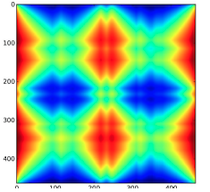
\includegraphics[width=0.25\linewidth]{Comps/Images/Wang2015 Gramium Angular Summation Field (GASF).png}
    \caption{Wang 2015 Gramium Angular Summation Field}
    \label{Wang2015GASF}
\end{figure}

\begin{figure}[ht]
    \centering
    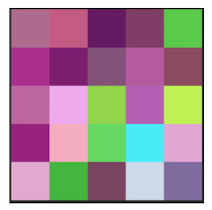
\includegraphics[width=0.25\linewidth]{Comps/Images/Basu2022 peak w:decline.png}
    \caption{Basu 2022 Financial Peak with Decline}
    \label{Basu2022FPwD}
\end{figure}

Since then various implementations have been used to create images suitable for classification.
Basu et al. \cite{Basu2022} converted financial time-series data of stocks into images by considering only certain features.
They used the High, Low, and Closing price of S\&P 500 index stocks, in a range of an odd-squared number of days (e.g. 9, 25, 49, etc.), to create RGB values of pixels.
Afterwards, they used a pre-trained Siamese Type Neural Network to classify their images, which can be seen in Figure~\ref{Basu2022FPwD}.

Zhu et al. (2021) develop Image Generator for Tabular Data (IGTD), whose conversion process consisted of assigning features to pixel positions so similarity of features can be expressed by distance of pixels \cite{Zhu2021}. The algorithm searches for an optimized assignment by minimizing the difference between the ranking of distances between features and the ranking of distances between their assigned pixels in the image.

Bazgir et al. (2020) developed REFINED (REpresentation of Features as Images with NEighborhood Dependencies) \cite{Bazgir2020}, which uses the Bayesian multidimensional scaling to create a map displaying the relative positions of the features, given a table of the distances between them. The features are then assigned to image pixels according to the mapping and a hill climbing algorithm is applied to locally optimize the arrangement of feature positions in the image.

Ma et al. (2018) developed OmicsMapNet to convert gene expression data of cancer patients into 2-D images for the prediction of tumor grade using CNNs \cite{Ma2018}. OmicsMapNet utilizes annotated genes to construct images via TreeMap, so that genes with similar molecular functions are closely located in the image, in a similar fashion to the previous two implementations.

\begin{figure}[ht]
    \centering
    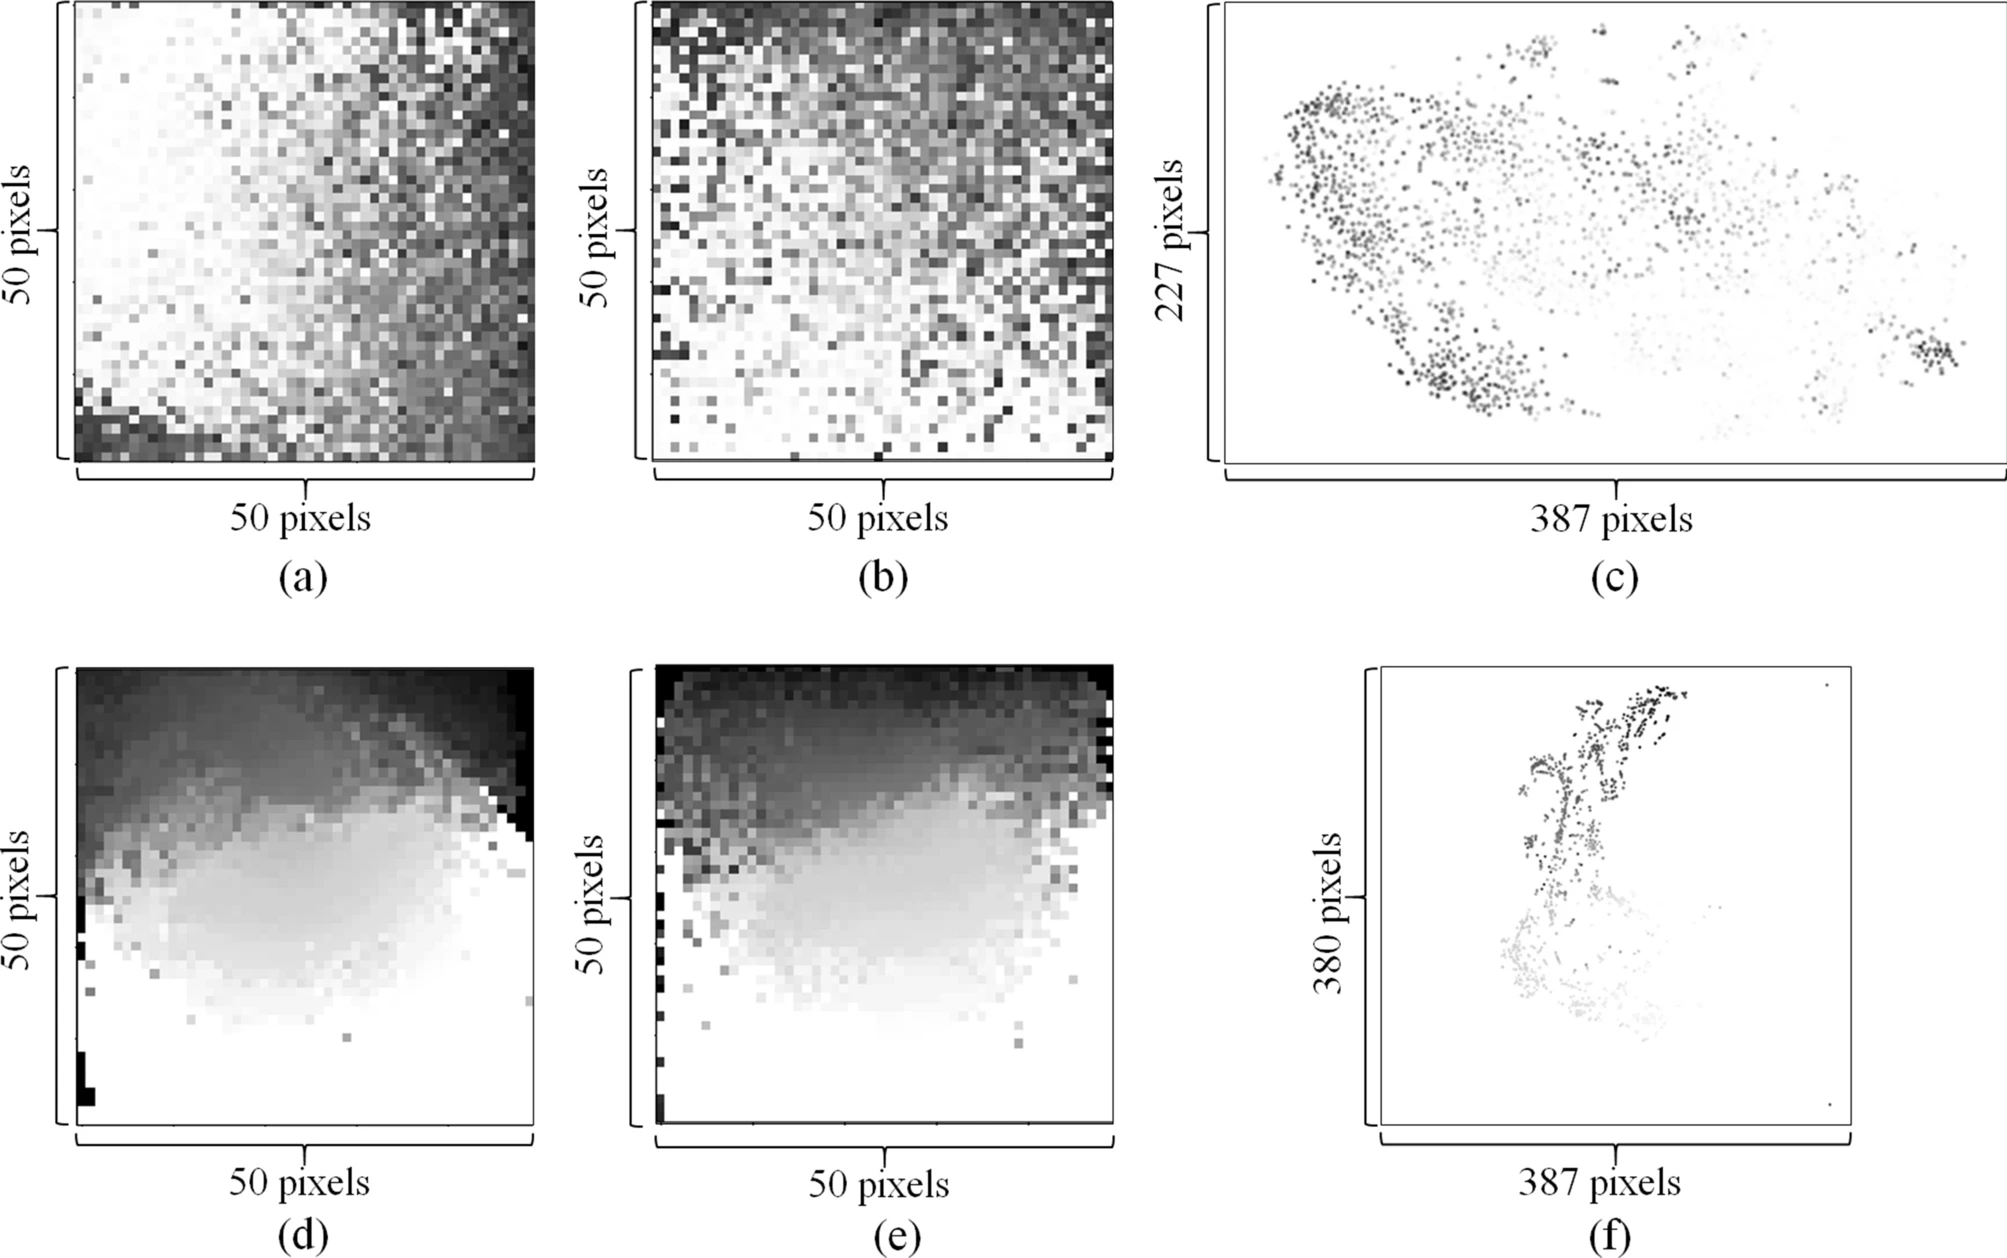
\includegraphics[width=0.8\linewidth]{Comps/Images/IGTD_REFINED_DEEPINSIGHT_COMPARISON.png}
    \caption{a–c are image representations of the gene expression profile of the SNU-61 cell line generated by IGTD, REFINED, and DeepInsight, respectively. d–f are image representations of molecular descriptors of Nintedanib, generated by IGTD, REFINED, and DeepInsight, respectively.\cite{Zhu2021}}
    \label{Zhu2021Comparison}
\end{figure}

Lastly, the method implemented in Buturovi{\'c} et al. (2020) had similarities to some of the implementations in terms of data or method.
Their goal was to classify bacterial and viral infections from blood samples \cite{Buturovic2020} and similarly to Basu et al. (2022), they used sequences of odd-square length but converted their data into a kernel.
A kernel, also known as convolution matrix or mask, is a small matrix used to create a filter on an image.
This happens by a taking the convolution matrix, usually a 3x3 or 5x5 matrix, and iteratively convoluting it with every 3x3 or 5x5 pixel segment of a base image, such as a rose.

% [Buturovi{\'c} 2020 Rose Image with filters]

\begin{figure}[ht]
    \centering
    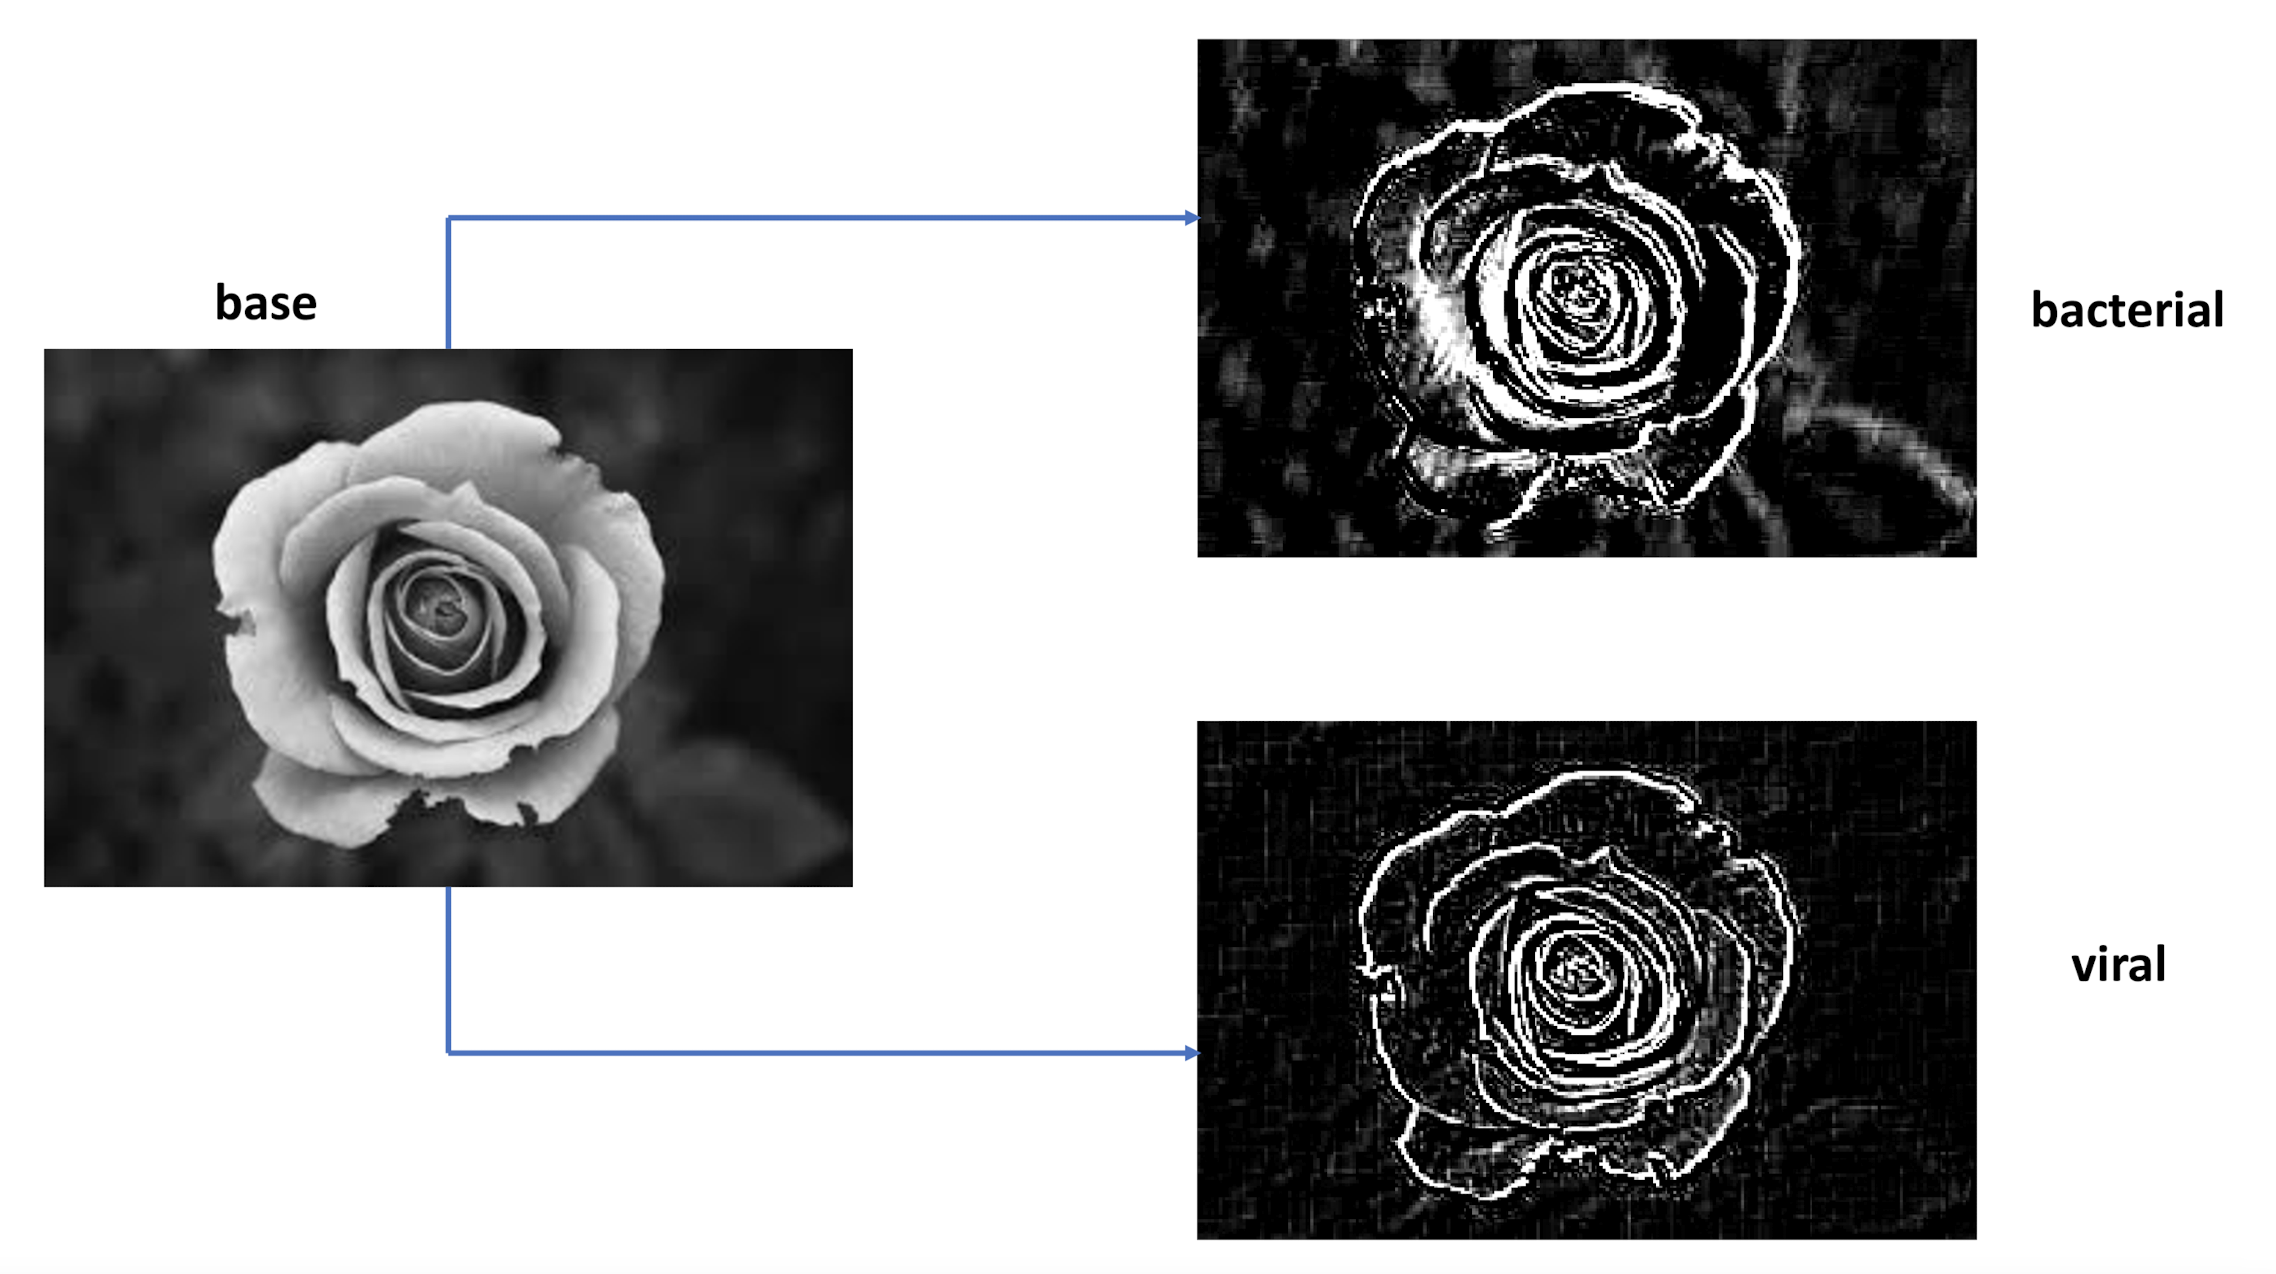
\includegraphics[width=0.8\linewidth]{Comps/Images/Butorović2020 Rose.png}
    \caption{Buturovi{\'c} 2020 Rose Image with filters}
    \label{Buturovic2020RwF}
\end{figure}

The convolution process will be discussed more in the section 3 of this review. The resulting filtered image (Figure~\ref{Buturovic2020RwF}) is used with a default ResNet model to classify them. This study showed that unoptimized CNN can achieve the same level of accuracy as optimized CNNs. Yet it also left some questions unanswered such as the impact of different base images, if a set of base images could be used instead of just one, and especially, what kind of results could be achieved by an optimized CNN. These questions are part of the main considerations for this project.

\section{Technical Background}

This implementation will require knowledge of both CNN and non-CNN models in order to compare the efficacy of each. Buturovi{\'c} et al. (2020) implemented 6 different non-CNN models for comparison with ResNet: XGBoost, LightGBM, SVM with linear and RBF kernel, multi-layer perceptron (MLP) and regularized logistic regression. In terms of comparison, at least one or two optimized non-CNN algorithms will be implemented. Which ones will be chosen after further investigation of the non-CNN models implemented in other studies and answering questions about their strengths, weaknesses, and in what areas may we want to choose one over another? However, Ma et al. (2018), Bazgir et al. (2020), and Zhu et al. (2021) each seem to have their implementations available to the public, so comparisons with other tabular conversion methods also exists as an avenue.

It is likely that the focus of this project will use the kernel method for conversion. Kernels work by creating a copy of an image with a filter applied using the underlying matrix structure of images. This may be a little difficult to understand at first so let’s consider an example.

% Convolution matrix for Gaussian blur
Let $A$ be a sample matrix of pixels, $C$ be the convolution matrix, and $R$ be our resulting convoluted matrix. Let each be a $n \times n$ matrix where $n = 3$. Our convolution can be represented by $A \cdot C = R$. Consider the following example where $A \cdot C$ is given by,
\[
    \begin{bmatrix}
      1 & 2 & 3 \\
      4 & 5 & 6 \\
      7 & 8 & 9
    \end{bmatrix}
    \cdot
    \frac{1}{16}
    \begin{bmatrix}
      1 & 2 & 1 \\
      2 & 4 & 2 \\
      1 & 2 & 1
    \end{bmatrix}\]

The kernal used here is the one that approximates the Gaussian blur filter of an image. The convolution of $A$ with respect to $C$ can be computed by

\begin{multline*}
    \sum_{i=0}^{n-1}\sum_{j=0}^{n-1} (A_{ij}*C_{ij}) = 1(2) + 2(2) + 3(1) + 4(2) + 5(4) \\
    + 6(2) + 7(1) + 8(2) + 9(1) \\
\end{multline*}
This sum is equal to $81$ and $R$ will become the following:
\[
    =
    \frac{1}{16}
    \begin{bmatrix}
      -- & -- & -- \\
      -- & 81 & -- \\
      -- & -- & --
    \end{bmatrix}
\]

The blank ($--$) spaces representing the empty spaces. These spaces will be filled as the convolution matrix iterates through the different pixel sub-matrices of an image.

Using a method such as this, this project aims to develop off Buturovi{\'c} 2020’s research.
A main development will be to implement ResNet on a new dataset, test the performance on metrics such as accuracy and time, and then see the difference in performance when the model when optimized.
The optimization process will need to be planned out and different methods will need to be weighed against each other.
However, Dr. Basu, of Basu et al. 2022, has suggested using a random forest algorithm with the CNN as part of the optimization process.
A random forest tree creates multiple decision trees and searches for the best feature among a random subset of features, which increases the diversity of the results.
Finally, in relation to kernels, it would be desirable to understand the different kinds of convolution matrices and the effect that each one has on an image as well as if some are more effective than others at classification.

\printbibliography 

\end{document}